\lstinputlisting[language=bash,basicstyle=\small]{python_codes/fieldstone_10/keywords}

\begin{center}
Code at \url{https://github.com/cedrict/fieldstone/tree/master/python_codes/fieldstone_10}
\end{center}

\par\noindent\rule{\textwidth}{0.4pt}
%%%%%%%%%%%%%%%%%%%%%%%%%%%%%%%%%%%%%%%%%%%%%%%%%%%%%%%%%%%%%%%%%%%%%%%%%%%%%%%%%%%%%%%%%%%%

%----------------------------------------------------------
\subsection*{Manufactured solution ({\tt experiment=5})}

It is described in Section~\ref{ss:mms3Dgen}.
The velocity and pressure fields are:
\begin{eqnarray}
u(x,y,z) &=& x(1-x)(1-2y)(1-2z)\\
v(x,y,z) &=& (1-2x) y(1-y) (1-2z) \\
w(x,y,z) &=& -2(1-2x)(1-2y)z(1-z) \\
p(x,y,z) &=& (2x-1)(2y-1)(2z-1)
\end{eqnarray}
This flow field has the built-in property that there is no flux through the 
boundaries. 

\begin{center}
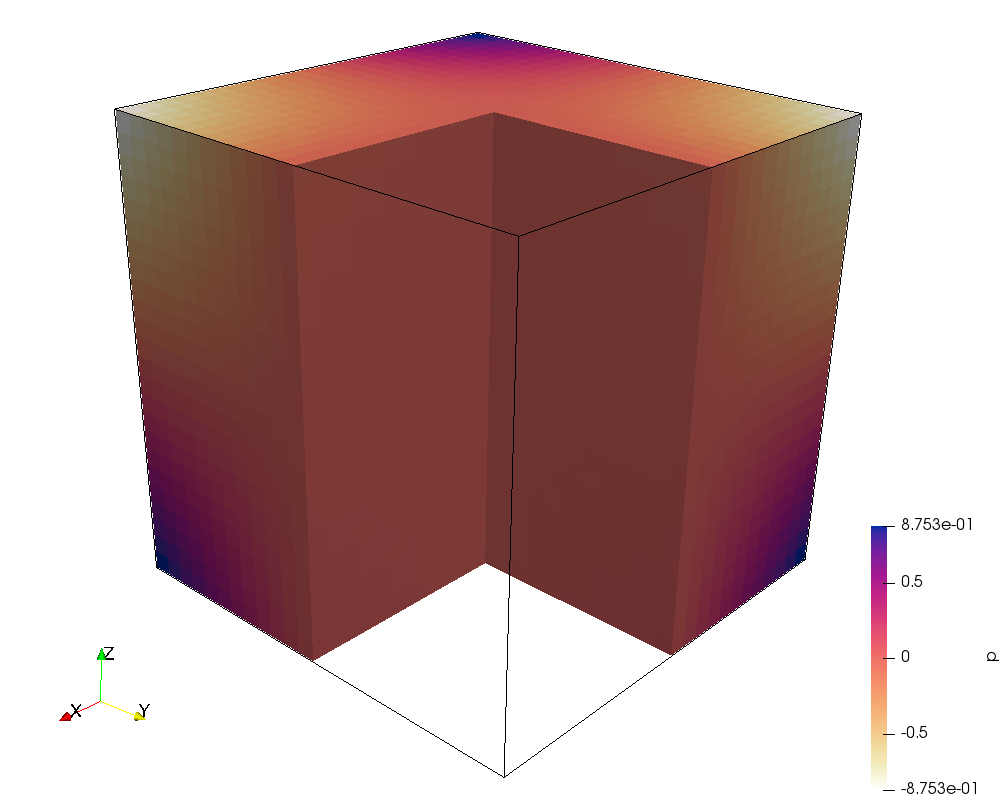
\includegraphics[width=5.6cm]{python_codes/fieldstone_10/results/exp5/press}
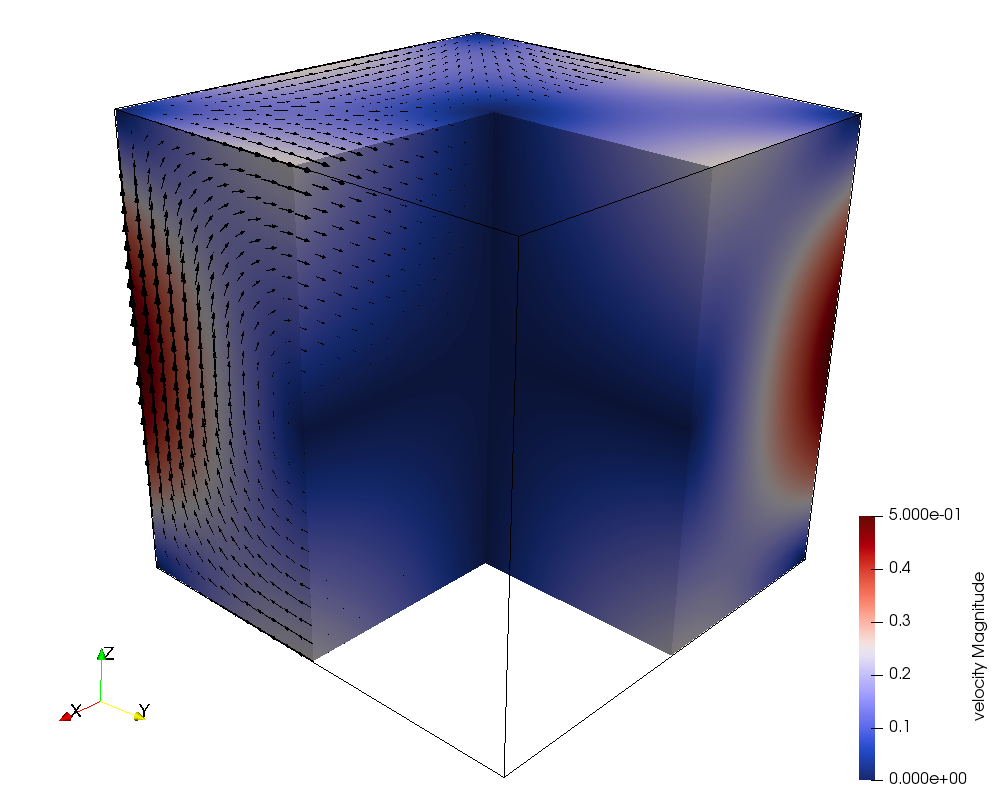
\includegraphics[width=5.6cm]{python_codes/fieldstone_10/results/exp5/vel}
\end{center}

\begin{center}
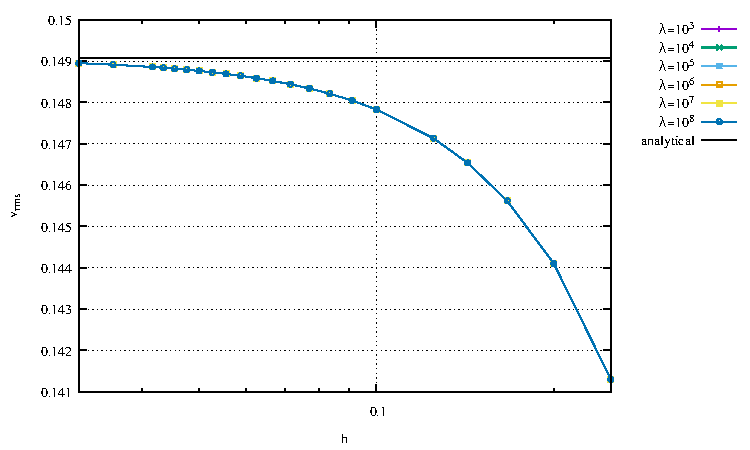
\includegraphics[width=5.6cm]{python_codes/fieldstone_10/results/exp5/vrms}
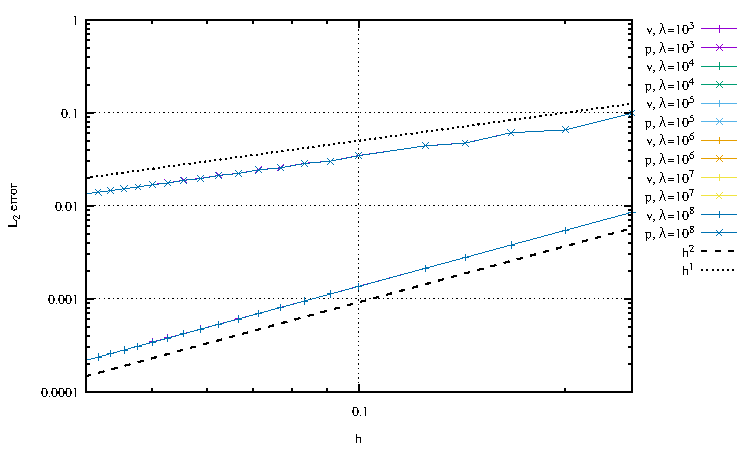
\includegraphics[width=5.6cm]{python_codes/fieldstone_10/results/exp5/conv}
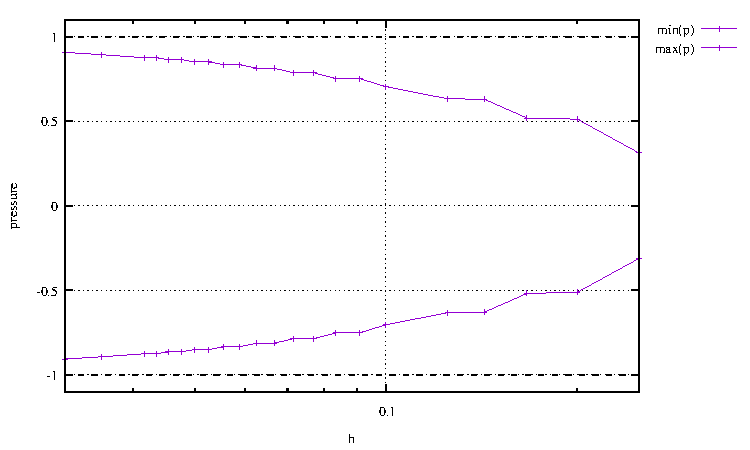
\includegraphics[width=5.6cm]{python_codes/fieldstone_10/results/exp5/p_stats}
\end{center}
We recover the expected second order velocity error convergence 
and first order pressure error convergence. 
Surprisingly, we find that the results are not sensitive to the value of the penalty parameter $\lambda$.



%------------------------------
\subsection*{Stokes sphere}

The domain is a unit cube. Free slip boundary conditions 
are imposed on all sides. The mesh counts 
nelx*nely*nelz=nel elements and 
nnx*nny*nnz=NV nodes.
The density and the viscosity are prescribed in the domain 
by means of two functions:
the density is set to $1+\delta \rho$ inside a sphere of radius 0.123456789 centered 
at (0.5,0.5,0.5) and 1 outside. The viscosity is 1000 inside the sphere
and 1 outside.  The gravity vector is set to $\vec{g}=(0,0,-1)$.
This is the benchmark presented in Section~\ref{ss:stokes_sphere_3D}.

The FE matrix size grows even faster now than in the previous 2D case so
choosing the right matrix storage is of paramount importance. 

Three experiments are carried out:
\begin{enumerate}
\item[Exp.~1:] the one described above.
Free slip or no slip boundary conditions.
We see that the pressure field is dominated by the lithostatic signal.
\item[Exp.~2:] same as experiment 1, but a reference density of 1 is substracted to all densities, so that 
the sphere density is 1 and the density of the surrounding fluid is now 0. In essence, we remove a
'background' density which does not participate in the flow generation, and thereby get rid of the 
lithostatic signal of the pressure.
Free slip or no slip boundary conditions.
\item[Exp.~3:] same as experiment 2, but the top boundary is now open (free surface)
\end{enumerate} 

\begin{center}
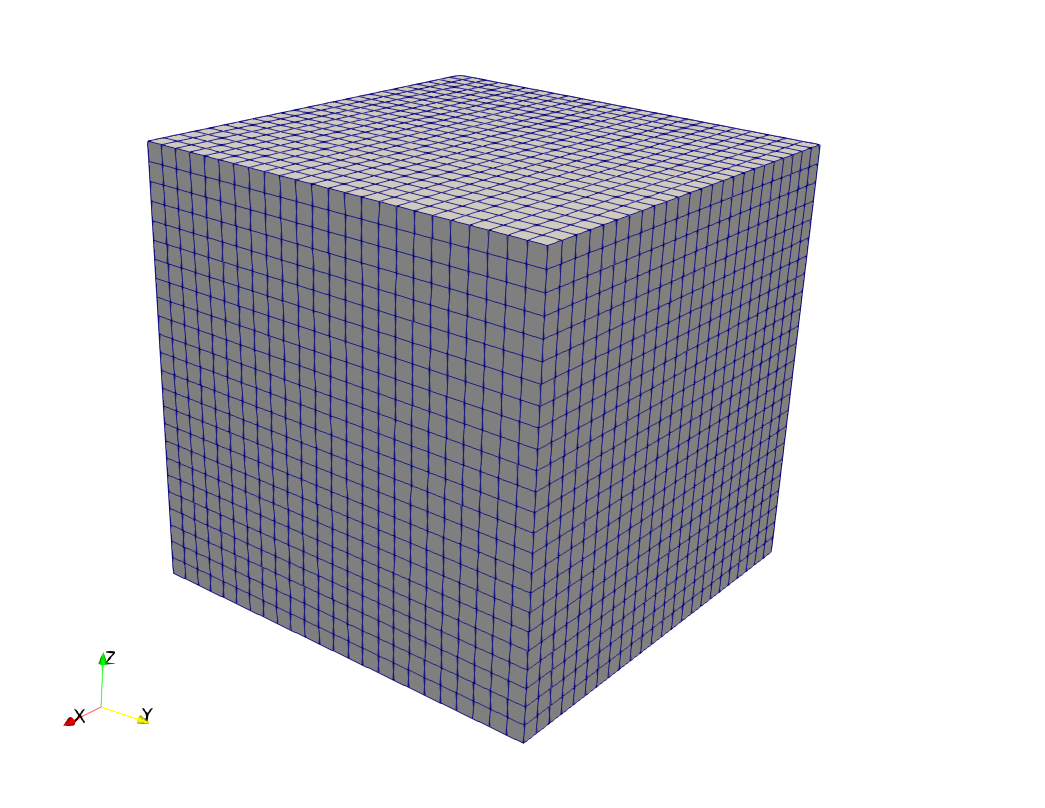
\includegraphics[width=5cm]{python_codes/fieldstone_10/results/exp1/grid}
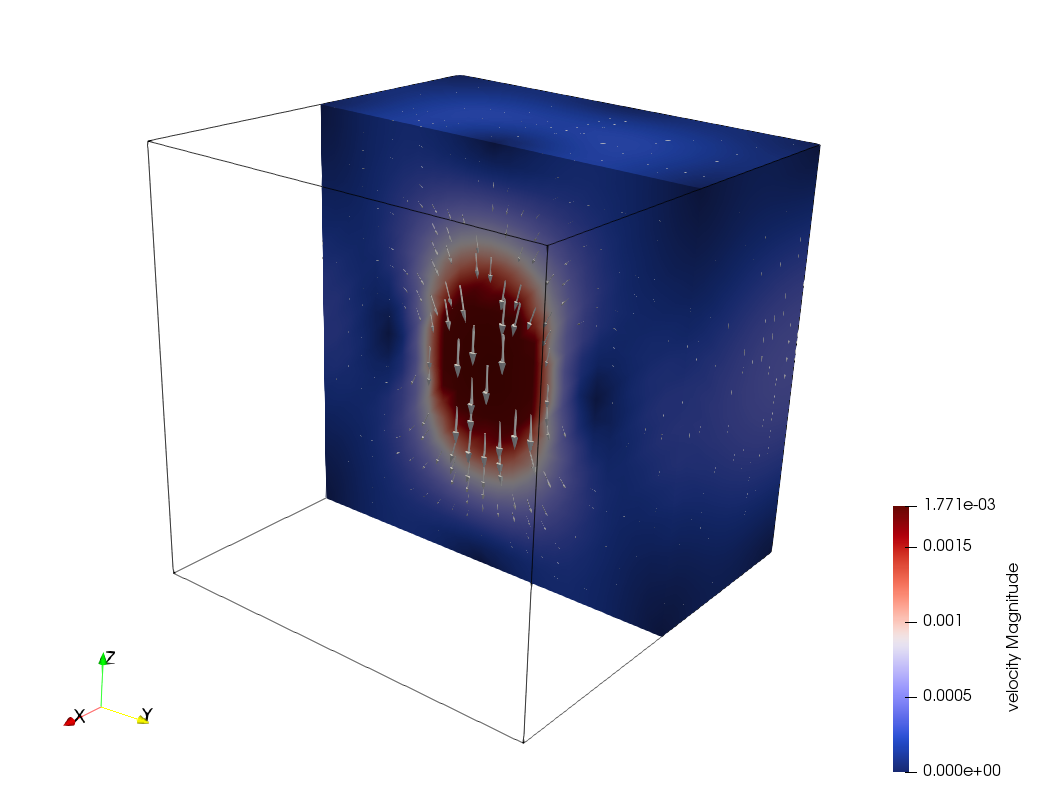
\includegraphics[width=5cm]{python_codes/fieldstone_10/results/exp1/vel}
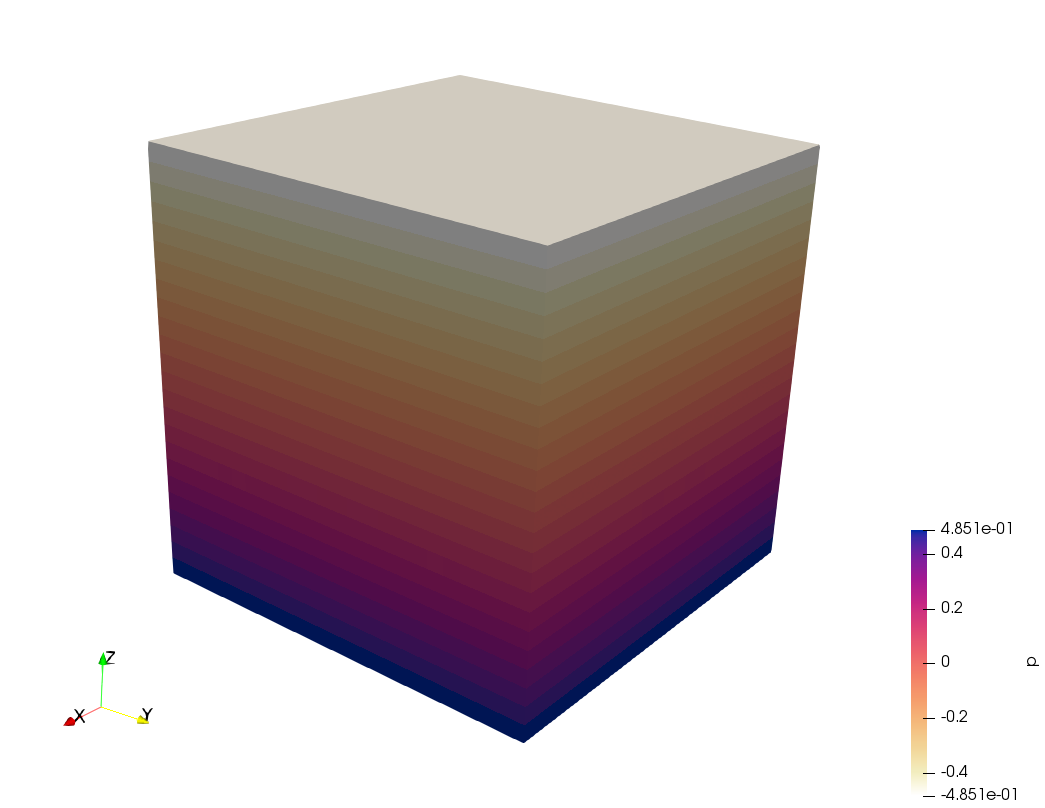
\includegraphics[width=5cm]{python_codes/fieldstone_10/results/exp1/press}\\
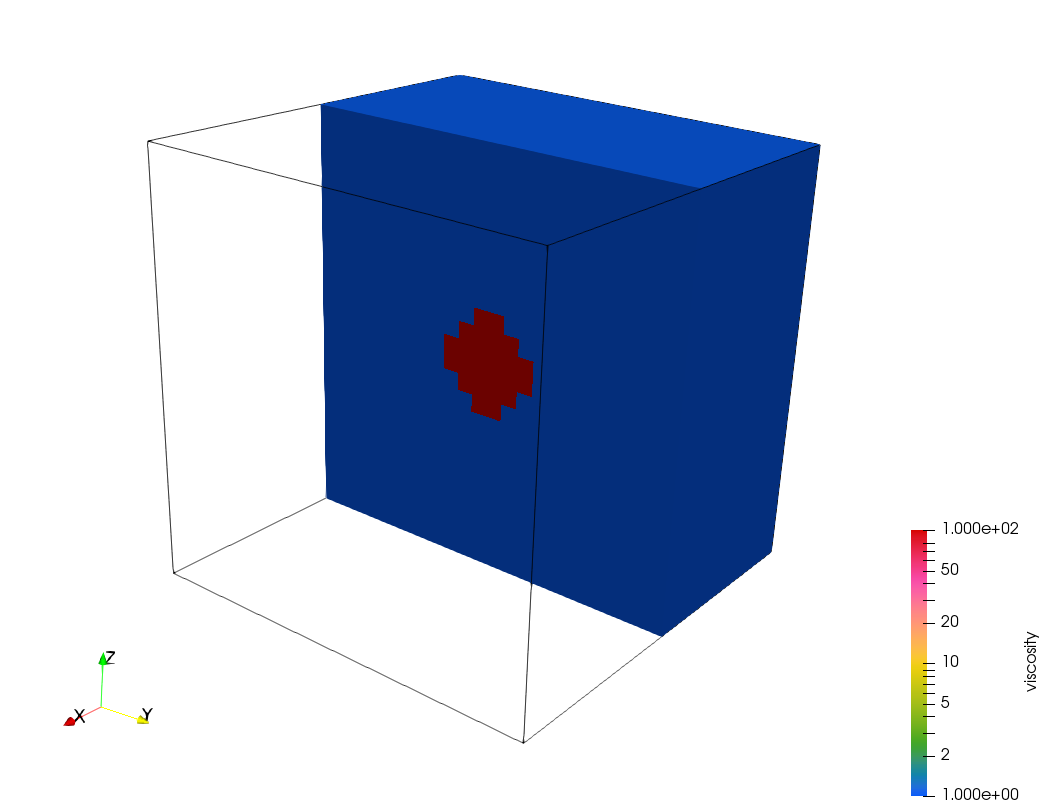
\includegraphics[width=5cm]{python_codes/fieldstone_10/results/exp1/visc}
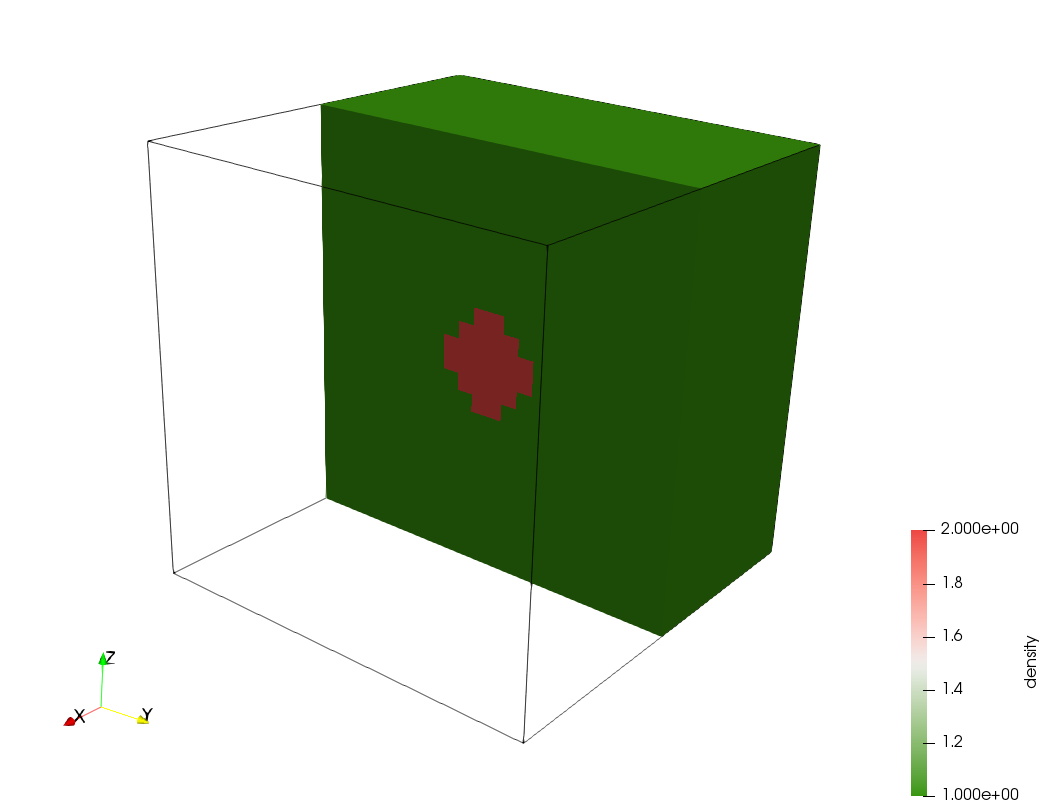
\includegraphics[width=5cm]{python_codes/fieldstone_10/results/exp1/dens}\\
{\small Exp.~1: resolution $24\times 24\times 24$}
\end{center}

\begin{center}
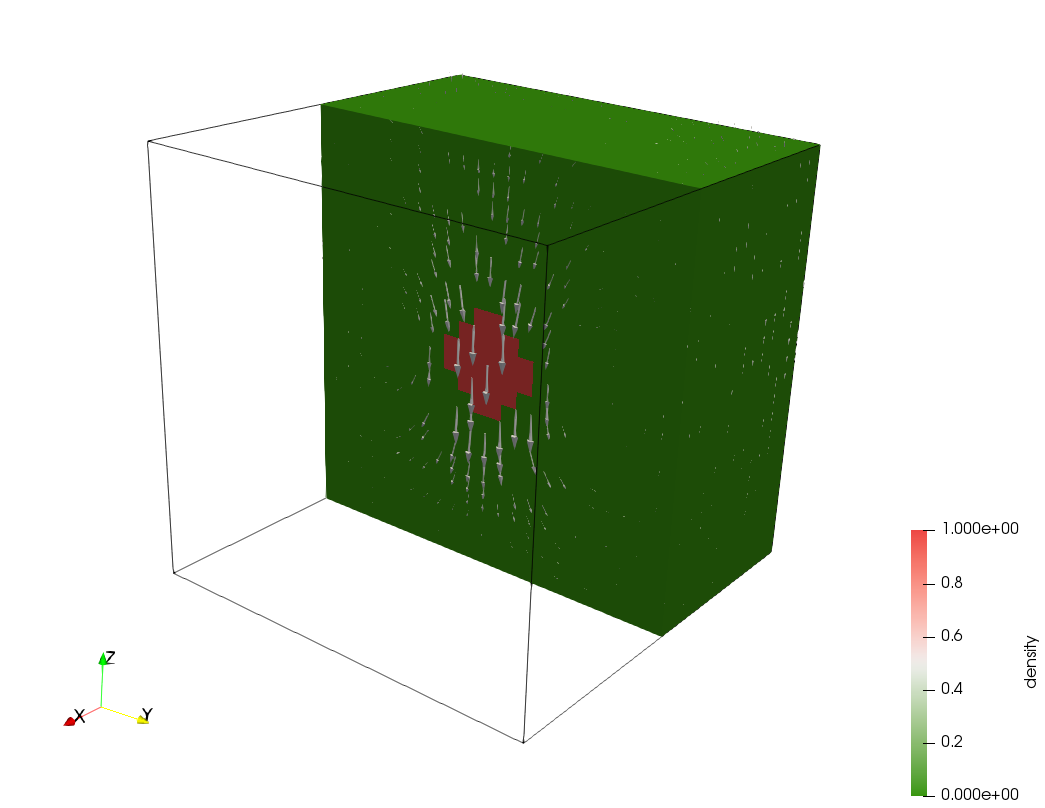
\includegraphics[width=5cm]{python_codes/fieldstone_10/results/exp2/dens_2}
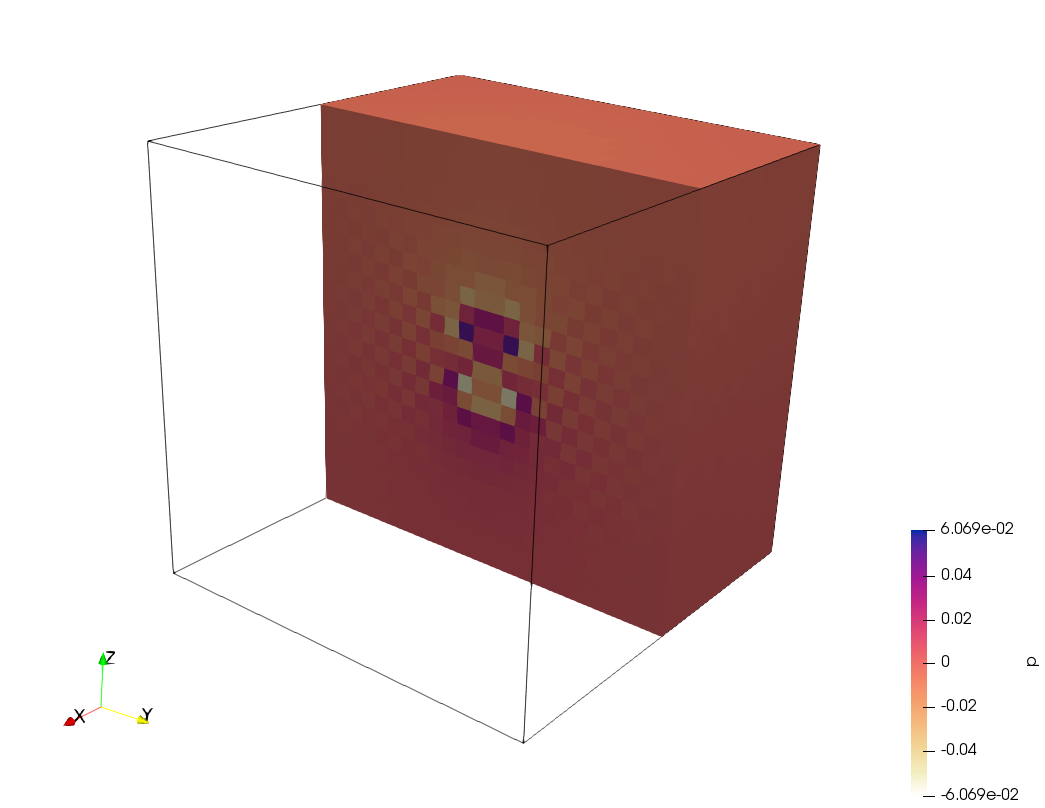
\includegraphics[width=5cm]{python_codes/fieldstone_10/results/exp2/press_2}\\
{\small Exp.~2: Density and pressure fields. Resolution 24x24x24}
\end{center}


\begin{center}
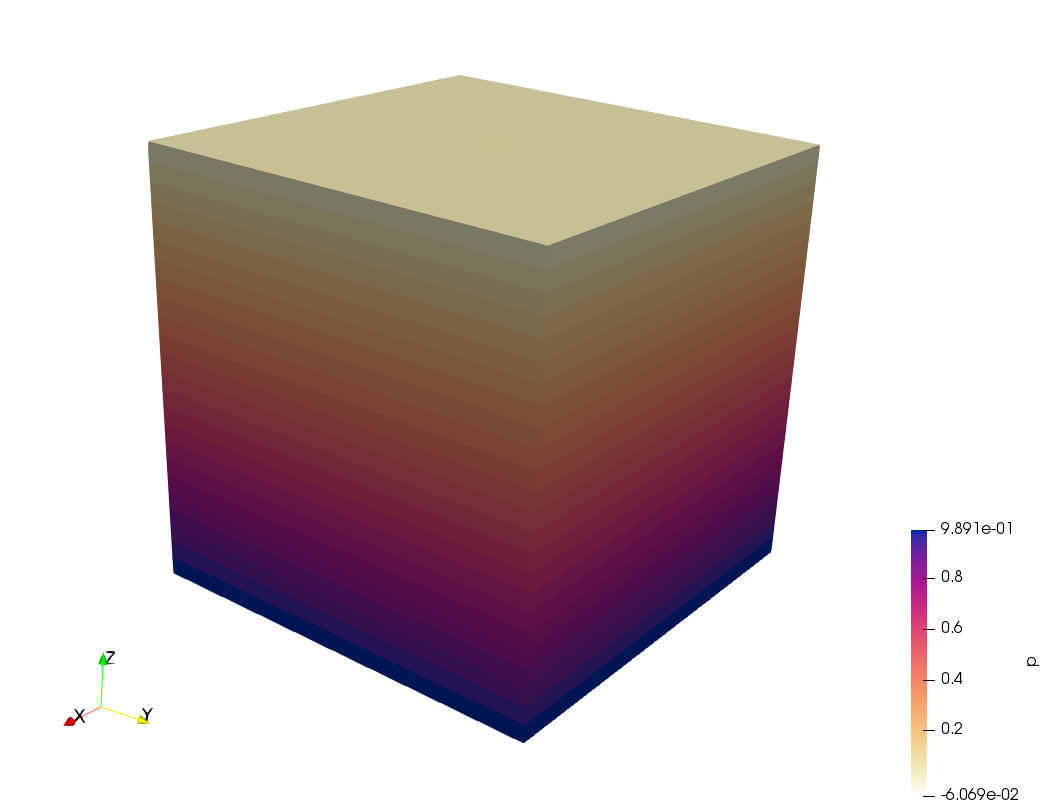
\includegraphics[width=5cm]{python_codes/fieldstone_10/results/exp3/press_3}
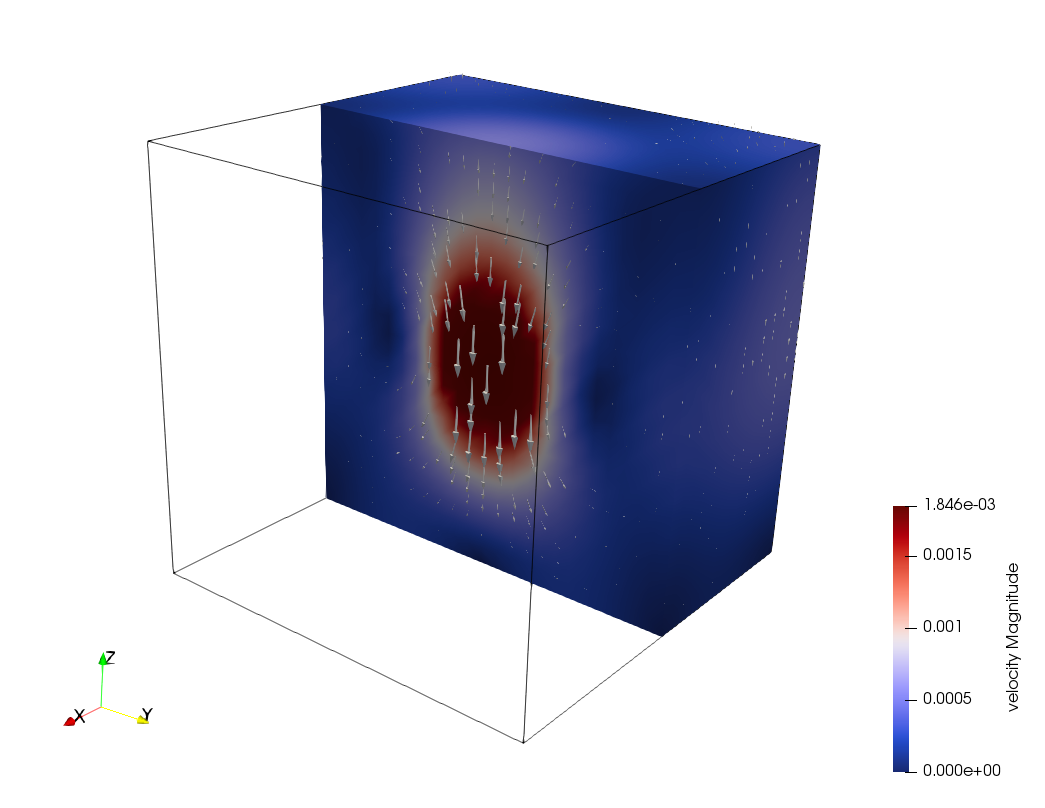
\includegraphics[width=5cm]{python_codes/fieldstone_10/results/exp3/vel_3}\\
{\small Exp.~3: pressure and velocity fields. Resolution 24x24x24}
\end{center}

\begin{center}
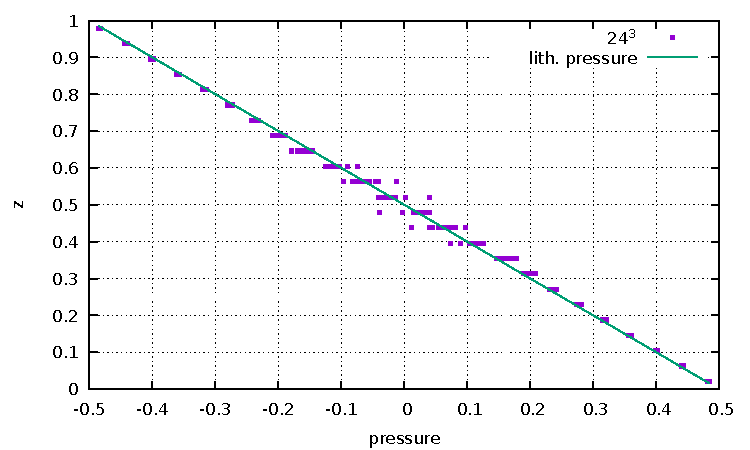
\includegraphics[width=5.6cm]{python_codes/fieldstone_10/results/exp1/pressure.pdf}
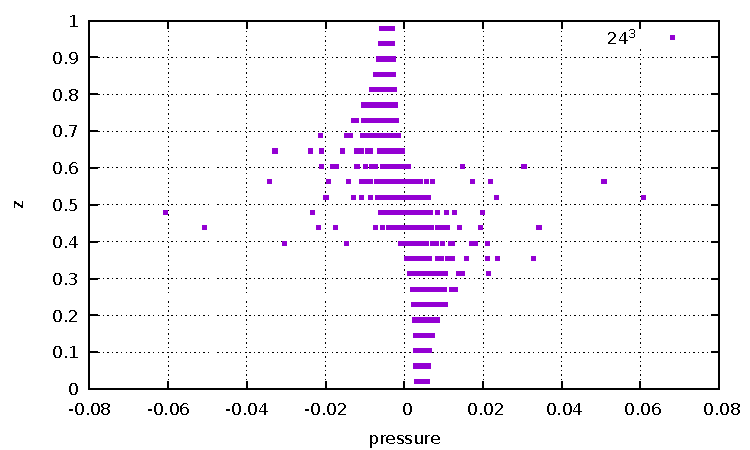
\includegraphics[width=5.6cm]{python_codes/fieldstone_10/results/exp2/pressure.pdf}
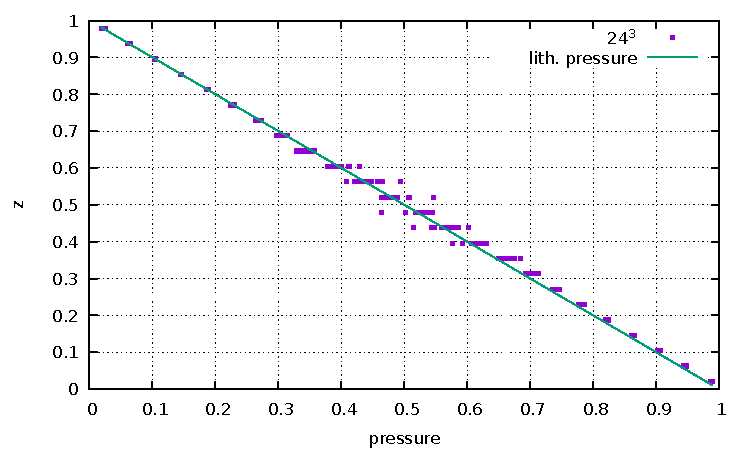
\includegraphics[width=5.6cm]{python_codes/fieldstone_10/results/exp3/pressure.pdf}\\
{\captionfont Elemental pressure for all elements as a function of their vertical 
(middle) coordinate for (from left to right) experiments 1, 2 and 3. }
\end{center}

Note that a similar fortran code is present in the folder. 

If the option 'quarter' is true, then the model takes advantage of the symmetries 
of the problem and runs it in a quarter of the original domain, so that 
the domain is then $0.5\times 0.5 \times 1$. Measurements/results are identical 
to the full cube ones, but at a much lower cost.

\begin{center}
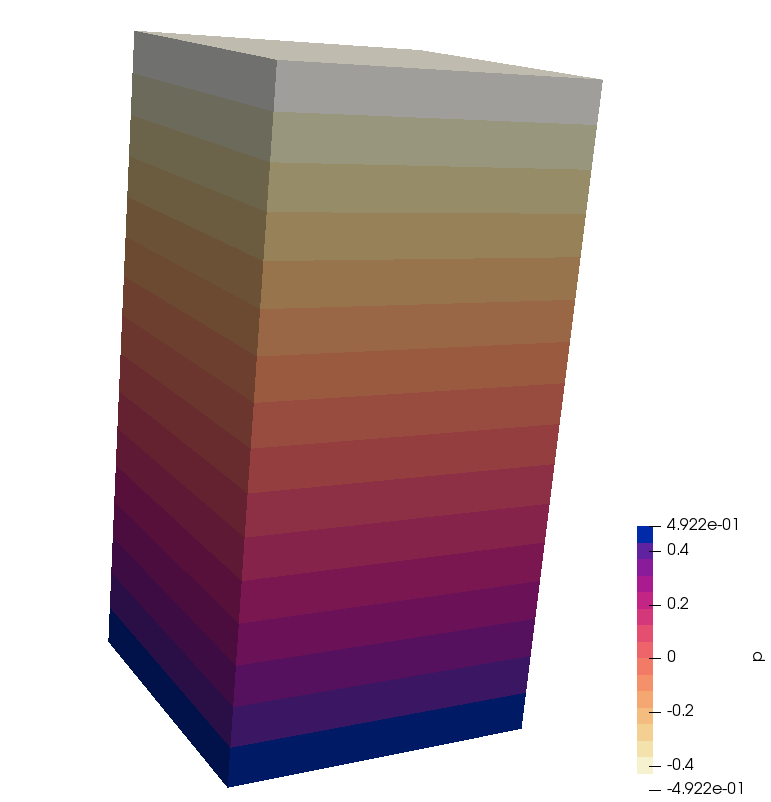
\includegraphics[width=4cm]{python_codes/fieldstone_10/results/quarter_FS/press}
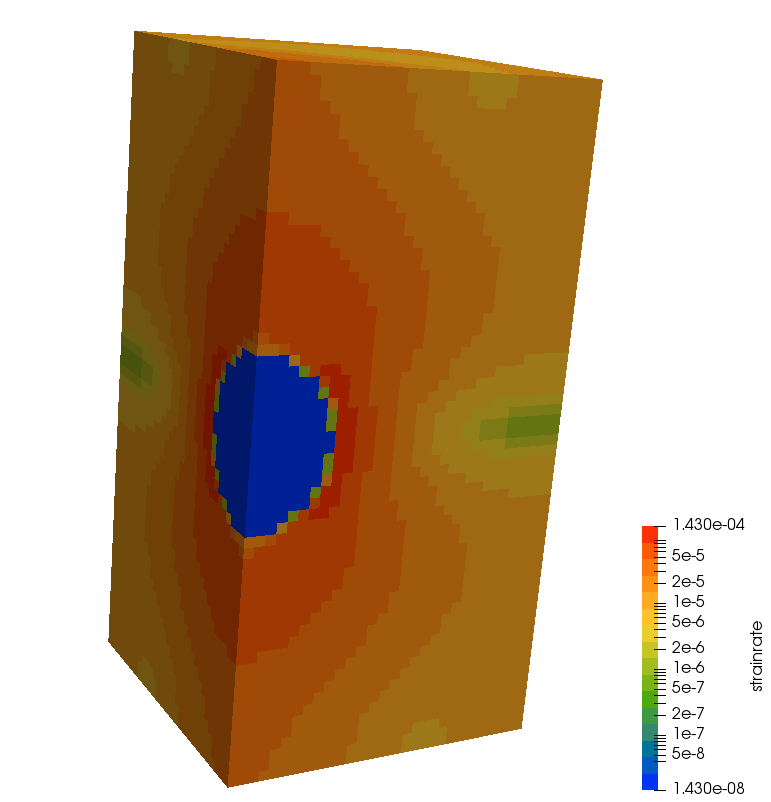
\includegraphics[width=4cm]{python_codes/fieldstone_10/results/quarter_FS/sr}
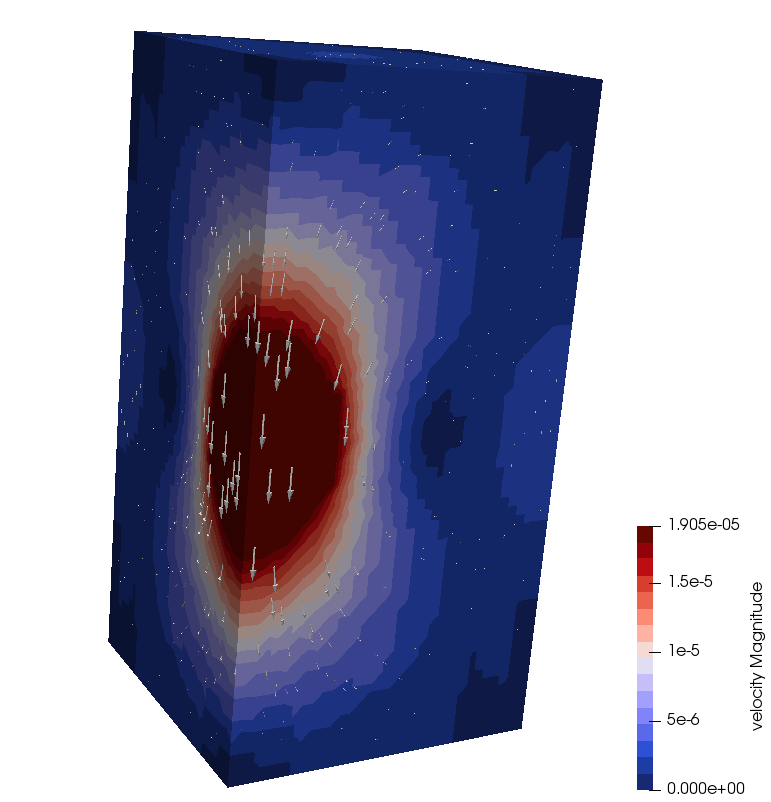
\includegraphics[width=4cm]{python_codes/fieldstone_10/results/quarter_FS/vel}
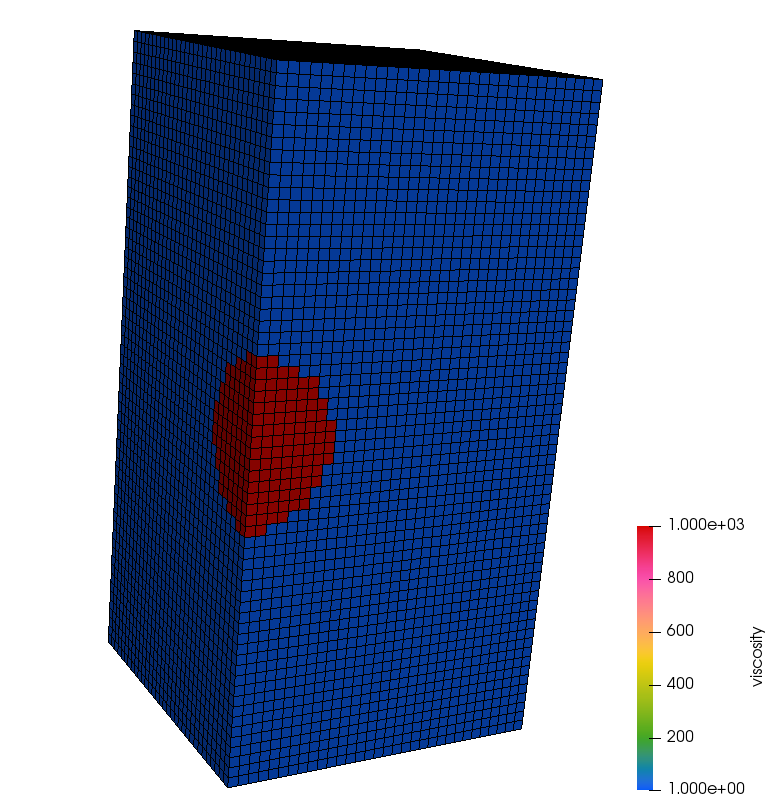
\includegraphics[width=4cm]{python_codes/fieldstone_10/results/quarter_FS/eta}\\
{\captionfont Resolution $32\times 32\times 64$ - FS}
\end{center}




\begin{center}
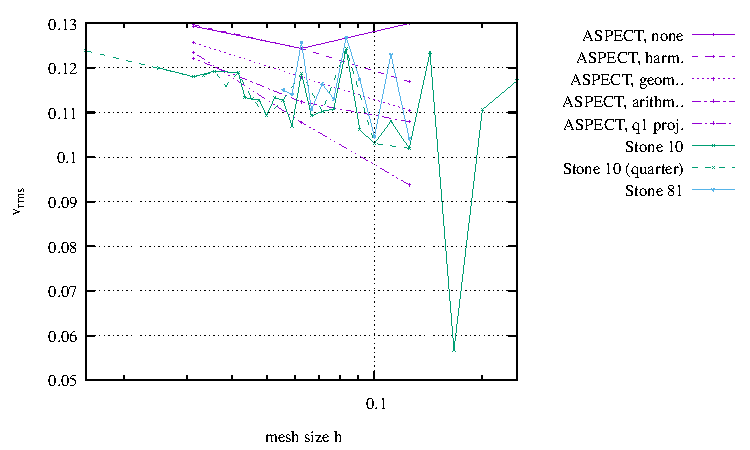
\includegraphics[width=7cm]{images/stokes_sphere3D/vrms_FS}
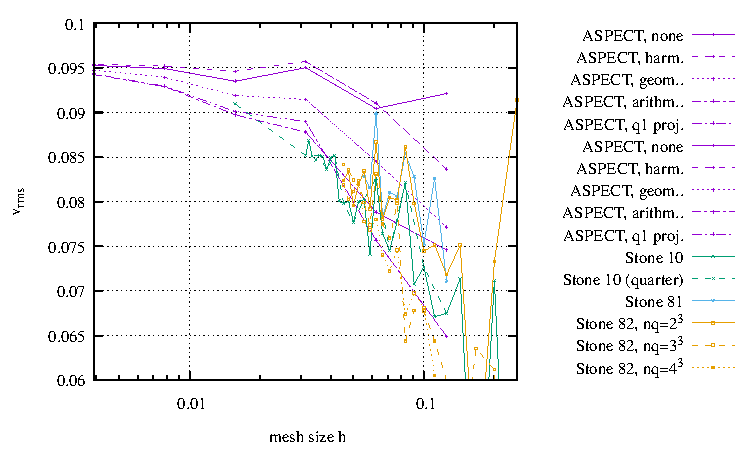
\includegraphics[width=7cm]{images/stokes_sphere3D/vrms_NS}\\
{\captionfont Left: FS; Right: NS. Results obtained with this stones and other ones, as well as ASPECT.
See Section~\ref{ss:stokes_sphere_3D} for all results.}
\end{center}
